\chapter{Template Method模式}
\section{Template Method模式概念}
\subsection{Template Method定义}
\noindent \textbf{模板方法:}定义一个操作中的算法骨架,而将算法的一些步骤延迟到子类中,使得子类可以不改变该算法结构的情况下重定义该算法的某些特定步骤。它是一种类行为型模式。
\\ 另一理解:在父类中定义处理流程的框架,但在子类中实现具体处理的模式。
\subsection{优点}
\begin{itemize}
	\item 它封装了不变部分,扩展可变部分。它把认为是不变部分的算法封装到父类中实现,而把可变部分算法由子类继承实现,便于子类继续扩展。
	\item 它在父类中提取了公共的部分代码,便于代码复用。
	\item 部分方法是由子类实现的,因此子类可以通过扩展方式增加相应的功能,符合开闭原则。
\end{itemize}
\subsection{缺点}
\begin{itemize}
	\item 对每个不同的实现都需要定义一个子类,这会导致类的个数增加,系统更加庞大,设计也更加抽象。
	\item 父类中的抽象方法由子类实现,子类执行的结果会影响父类的结果,这导致一种反向的控制结构,它提高了代码阅读的难度。
\end{itemize}
\subsection{模式的角色}
\noindent \textbf{抽象类:}负责给出一个算法的轮廓和骨架。它由一个模板方法和若干个基本方法构成。
\begin{enumerate}
	\item \textbf{模板方法:}定义了算法的骨架,按某种顺序调用其包含的基本方法。
	\item \textbf{基本方法:}是整个算法中的一个步骤。
	\begin{itemize}
		\item 抽象方法:在抽象类中申明,由具体子类实现。
		\item 具体方法:在抽象类中已经实现,在具体子类中可以继承或重写它。
		\item 钩子方法:在抽象类中已经实现,包括用于判断的逻辑方法和需要子类重写的空方法两种。
	\end{itemize}
\end{enumerate}
\textbf{具体子类:}实现抽象类中所定义的抽象方法和钩子方法,它们是一个顶级逻辑的一个组成步骤。
\subsection{应用场景}
\begin{enumerate}
	\item 算法的整体步骤很固定,但其中个别部分易变时,这时候可以使用模板方法模式,将容易变的部分抽象出来,供子类实现。
	\item 当多个子类存在公共的行为时,可以将其提取出来并集中到一个公共父类中以避免代码重复。首先,要识别现有代码中的不同之处,并且将不同之处分离为新的操作。最后,用一个调用这些新的操作的模板方法来替换这些不同的代码。
	\item 当需要控制子类的扩展时,模板方法只在特定点调用钩子操作,这样就只允许在这些点进行扩展。
\end{enumerate}
\begin{figure}[!h]
	\centering
	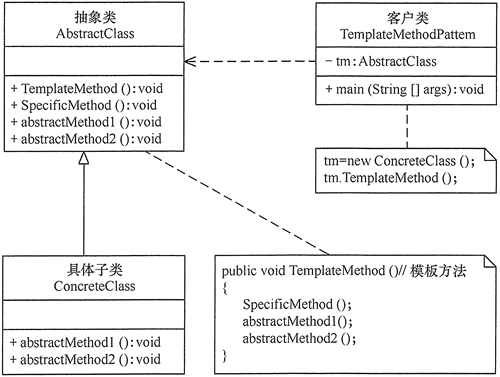
\includegraphics[width=0.8\textwidth]{image/3-1}
	\caption{模板方法模式的结构图}
\end{figure}
\section{模板方法——例一}
\begin{lstlisting}
public abstract class AbstractDisplay {
	public abstract void open();
	public abstract void print();
	public abstract void close();
	public final void display() {
		open();
		for (int i = 0; i < 5; i++) {
			print();
		}
		close();
	}
}
\end{lstlisting}
\begin{lstlisting}
public class CharDisplay extends AbstractDisplay{
	private char ch;
	public CharDisplay(char ch) {
		this.ch = ch;
	}
	public void open() {
		System.out.print("<<");
	}
	public void print() {
		System.out.print(ch);
	}
	public void close() {
		System.out.println(">>");
	}
}

public class StringDisplay extends AbstractDisplay {
	private String string;
	private int width;

	public StringDisplay(String string) {
		this.string = string;
		this.width = string.getBytes().length;
	}
	public void open() {
		printLine();
	}
	public void print() {
		System.out.println("|" + string + "|");
	}
	public void close() {
		printLine();
	}
	private void printLine() {
		System.out.print("+");
		for (int i = 0; i < width; i++) {
			System.out.print("-");
		}
		System.out.println("+");
	}
}
\end{lstlisting}
\begin{lstlisting}
public class Main {
	public static void main(String[] args) {
		AbstractDisplay d1 = new CharDisplay('H');
		AbstractDisplay d2 = new StringDisplay("Hello World");
		d1.display();
		d2.display();
	}
}
\end{lstlisting}
\begin{lstlisting}
//output
<<HHHHH>>
+-----------+
|Hello World|
|Hello World|
|Hello World|
|Hello World|
|Hello World|
+-----------+
\end{lstlisting}
\section{模板方法——例二}
\begin{lstlisting}
public class TemplateMethodPattern {
	public static void main(String[] args) {
		AbstractClass tm = new ConcreteClass();
		tm.TemplateMethod();
	}
}

//抽象类
abstract class AbstractClass {
	//模板方法
	public void TemplateMethod() {
		SpecificMethod();
		abstractMethod1();
		abstractMethod2();
	}
	//具体方法
	public void SpecificMethod() {
		System.out.println("抽象类中的具体方法被调用...");
	}
	public abstract void abstractMethod1(); //抽象方法1
	public abstract void abstractMethod2(); //抽象方法2
}

//具体子类
class ConcreteClass extends AbstractClass {
	public void abstractMethod1() {
		System.out.println("抽象方法1的实现被调用...");
	}
	public void abstractMethod2() {
		System.out.println("抽象方法2的实现被调用...");
	}
}
\end{lstlisting}
\section{模板方法扩展——钩子方法}
可以通过在具体子类中重写钩子方法 HookMethod1() 和 HookMethod2() 来改变抽象父类中的运行结果。
\begin{figure}
	\centering
	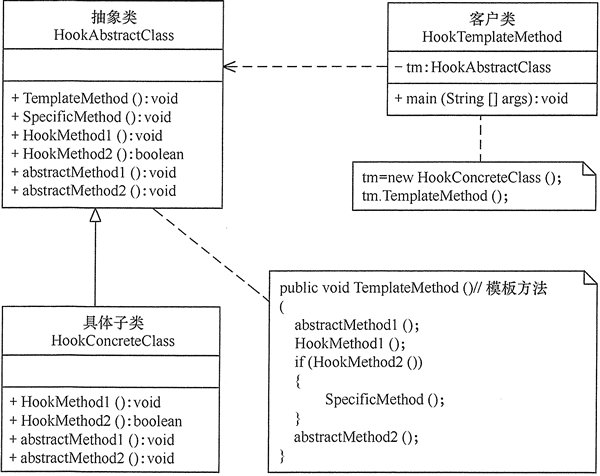
\includegraphics[width=0.8\textwidth]{image/3-2}
	\caption{含钩子方法的模板方法模式的结构图}
\end{figure}
\begin{lstlisting}
public class HookTemplateMethod {
	public static void main(String[] args) {
		HookAbstractClass tm = new HookConcreteClass();
		tm.TemplateMethod();
	}
}

//含钩子方法的抽象类
abstract class HookAbstractClass {
	//模板方法
	public void TemplateMethod() {
		abstractMethod1();
		HookMethod1();
		if (HookMethod2()) {
			SpecificMethod();
		}
		abstractMethod2();
	}

	//具体方法
	public void SpecificMethod() {
		System.out.println("抽象类中的具体方法被调用...");
	}
	
	//钩子方法1
	public void HookMethod1() {
	}
	
	//钩子方法2
	public boolean HookMethod2() {
		return true;
	}
	
	//抽象方法1
	public abstract void abstractMethod1();
	
	//抽象方法2
	public abstract void abstractMethod2();
}

//含钩子方法的具体子类
class HookConcreteClass extends HookAbstractClass {
	public void abstractMethod1() {
		System.out.println("抽象方法1的实现被调用...");
	}
	
	public void abstractMethod2() {
		System.out.println("抽象方法2的实现被调用...");
	}
	
	public void HookMethod1() {
		System.out.println("钩子方法1被重写...");
	}
	
	public boolean HookMethod2() {
		return false;
	}
}
\end{lstlisting}
\begin{lstlisting}
//output
抽象方法1的实现被调用...
钩子方法1被重写...
抽象方法2的实现被调用...
\end{lstlisting}
\section{扩展思路}
\begin{enumerate}
	\item 使用模板方法,可以是逻辑处理通用化;
	\item 在子类中实现父类中声明的抽象方法时,必须理解这些抽象方法被调用的时机,在不知道源代码,
	编写子类很困难。
	\item 父类保存子类实例优点:即使没有instanceof指定子类种类,程序也能正常工作,
	无论父类保存那个子类都能工作(里氏替换原则LSP)。
	\item 与其他模式区别:
	\begin{itemize}
		\item 工厂方法是将模板方法用于生成实例的一个经典例子;
		\item 模板模式可以使用继承改变程序的行为,因为模板模式在父类中定义程序行为框架,子类中决定具体的处理。
		\item 而策略模式使用委托改变程序的行为,与模板方法改变部分程序行为不同的是,策略模式用于替换整个算法。
	\end{itemize}
\end{enumerate}
\section{类的层次与抽象类}
理解类的层次通常站在子类角度思考:
\begin{itemize}
	\item 在子类中使用父类中定义的方法;
	\item 可以通过子类中增加方法以实现新的功能;
	\item 在子类中重写父类的方法可以改变程序的行为。
\end{itemize}
但站在父类思考:
\begin{itemize}
	\item 期待子类实现的抽象方法;
	\item 要求子类实现的抽象方法。
\end{itemize}
二者关系:父类承担大,子类灵活性降低;子类责任大,将会代码大量重复。